% 1977 年山东B卷第 11 题：隧道横断面（按源卷第 5 页布局）
% 上为半圆（半径 x，拱顶），下为矩形（高 y）；底部中央有宽 2x-1、高 0.5 的凸台阶，
% 台阶下基线画虚线；底部两段各标 0.5，台阶竖高标 0.5
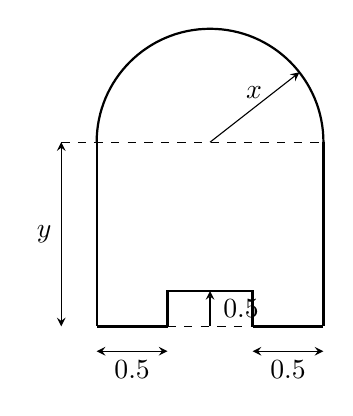
\begin{tikzpicture}[scale=0.9,>=stealth]
  % 半圆拱（圆心在拱弦线中点）
  \coordinate (L) at (-1.6,0);
  \coordinate (R) at (1.6,0);
  \draw[thick] (-1.6,0) arc[start angle=180,end angle=0,radius=1.6];
  % 拱弦线（虚线）
  \draw[dashed] (-2.1,0)--(1.6,0);
  % 半径 x 标注（箭头指向弧）
  \draw[->] (0,0)--(38:1.6);
  \node[above] at (0.62,0.48) {$x$};
  % 两侧竖墙
  \draw[thick] (-1.6,0)--(-1.6,-2.6);
  \draw[thick] (1.6,0)--(1.6,-2.6);
  % 底部：0.5 — 台阶（宽2x-1、高0.5）— 0.5
  \draw[thick] (-1.6,-2.6)--(-0.6,-2.6);
  \draw[thick] (-0.6,-2.6)--(-0.6,-2.1)--(0.6,-2.1)--(0.6,-2.6);
  \draw[thick] (0.6,-2.6)--(1.6,-2.6);
  % 台阶下基线（虚线）
  \draw[dashed] (-0.6,-2.6)--(0.6,-2.6);
  % 左侧高度 y 标注
  \draw[<->] (-2.1,0)--(-2.1,-2.6);
  \node[left] at (-2.1,-1.3) {$y$};
  % 底部左 0.5
  \draw[<->] (-1.6,-2.95)--(-0.6,-2.95);
  \node[below] at (-1.1,-2.95) {$0.5$};
  % 底部右 0.5
  \draw[<->] (0.6,-2.95)--(1.6,-2.95);
  \node[below] at (1.1,-2.95) {$0.5$};
  % 台阶高 0.5
  \draw[->] (0,-2.6)--(0,-2.1);
  \node[right] at (0.05,-2.35) {$0.5$};
\end{tikzpicture}
